Este simula la respuesta de un detector compuesto por un rastreador interno (The silicon Tracker), calorímetros electromagnéticos y de hadrones (\textbf{ECAL} y \textbf{HCAL}) y un sistema detector de muones (ver referencia \cite{de_favereau_delphes_2014}). Todos están organizados concéntricamente con una simetría cilíndrica alrededor del eje del haz. El usuario puede especificar el volumen activo del detector, la segmentación del calorímetro y la intensidad del campo magnético uniforme (Fig. \ref{delphes}). Cada subdetector tiene una respuesta específica, como se describe a continuación.

\begin{figure}[ht]
    \centering
    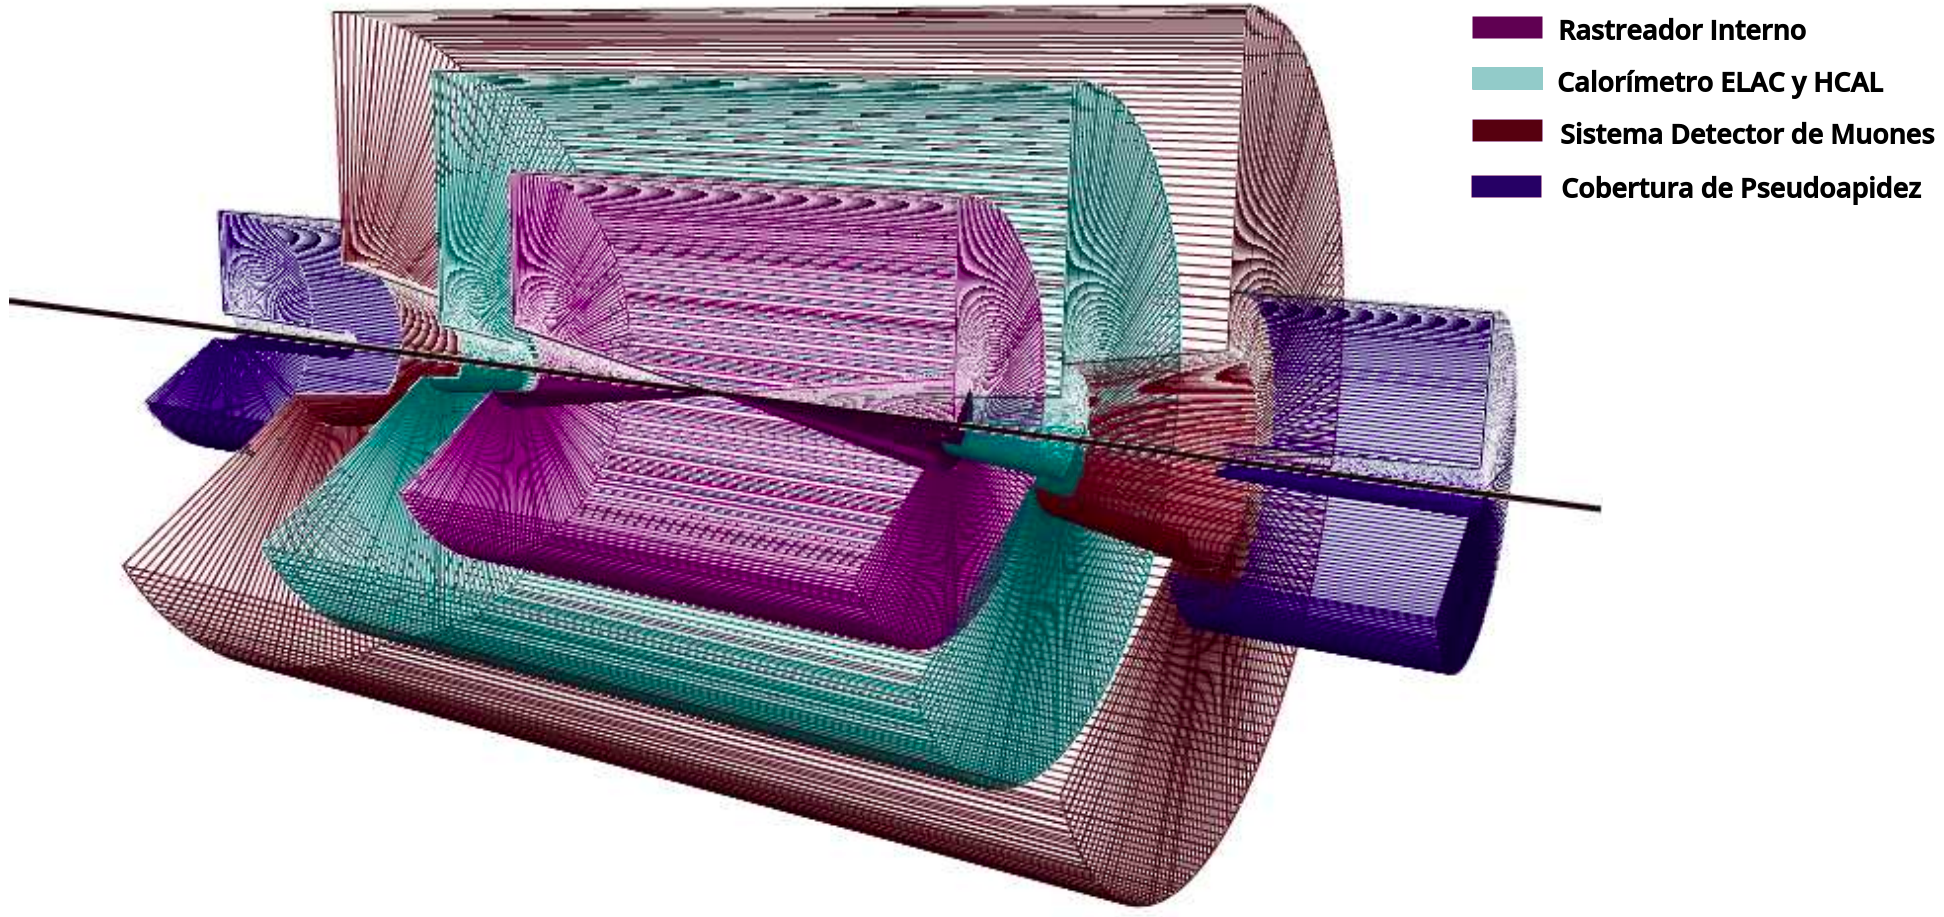
\includegraphics[width=1\textwidth]{Analisis_y_Resultados/imagenes/delphes.png}
    \caption{Perfil de diseño básico de la geometría del detector genérico asumido en Delphes. Adaptado de artículo de origen \cite{alwall_automated_2014}.}
    \label{delphes}
\end{figure}

En Delphes, la reconstrucción e identificación de objetos se basa en una serie de aproximaciones para acelerar sensiblemente el procedimiento y mantener una buena precisión. 

Los muones que se origina en la interacción, tiene cierta probabilidad de ser reconstruido, según la parametrización de eficiencia definida por el usuario. Esta probabilidad se desvanece fuera de la aceptación del rastreador, y para momentos de muón por debajo de algún umbral para rechazar partículas en bucle. El momento final del muón se obtiene mediante una mancha gaussiana del vector inicial de 4 momentos. La resolución es parametrizada en función de $p_T$ y $\eta$ implementada por el usuario.

El framework Delphes permite el acceso a datos de diferentes formatos de archivo (\textbf{ProMC}, \textbf{HEPMC}, \textbf{STDHEP} y \textbf{LHEF}). Los archivos de eventos provenientes de generadores externos \MC ~ son procesados primero por un lector, este convierte partículas estables en una colección de objetos universales, para luego ser procesada por una serie de módulos que comienzan con el módulo de fusión acumulada y terminan con el módulo de buscador de objetos único. Finalmente, Delphes permite al usuario almacenar y analizar eventos en un formato de árbol raíz al ejecutar DelphesHepMC tomando un archivo de configuración delphes\_card.tcl y realizando la simulación del detector en el archivo $*.hepmc$. La información sobre varios objetos \textbf{MC }(partículas) y objetos reconstruidos (jets, partículas reconstruidas), estas se guardan en un archivo $*.root$ en forma de árboles (``trees'') Delphes, el archivo de salida $*.root$ se puede abrir usando el mismo programa \ROOT.


%El aislamiento de un electrón, muón o fotón se realiza si la actividad en sus proximidades es lo suficientemente pequeña. Un objeto aislado tiene una pequeña probabilidad de originarse en un jet. Existen varias definiciones posibles para una variable de aislamiento, dependiendo del nivel particular de rechazo de señal a fondo que el analizador desea lograr. En Delphes se opto por uno simple, muy adecuado para experimentos con colisionadores de hadrones. Una definición alternativa, más adecuada para los experimentos, basada en variables esféricas, aunque aún no se ha implementado en Delphes, puede derivarse fácilmente de la presente. Además, la modularidad del marco permite al usuario otras definiciones, más adecuadas para diferentes experimentos o requisitos de análisis, o simplemente para no aplicar ningún criterio de aislamiento en los objetos finales.



